
\section{Premières mesures du temps d'exécution}

\subsection{Paramètres utilisés dans toute cette section}
Indiquez ici les valeurs de $m$ et $k$ avec lesquelles vous avez travaillé pour cette section. Indiquez également le ou les fichiers d'entrée utilisé(s) et la ou les valeur(s) de $n$ correspondantes. Indiquez également votre environnement de travail : système d'exploitation, compilateur (version), options de compilation, processeur, mémoire vive, etc. 

Pour chacune des sous-sections suivantes, indiquez le nombre de runs effectués pour soutenir vos résultats.

\subsection{Mise en évidence de la stochasticité de l'algorithme}
Montrez la variabilité obtenue dans les temps d'exécution en incluant un histogramme du temps CPU dans votre rapport (Figure \ref{fig:histo-variabilite}). Quantifiez cette variabilité en indiquant l'écart-type de ce temps d'exécution (sans oublier de préciser le nombre de runs sur lequel cet écart-type a été calculé). 

\begin{figure}[htbp]
	\begin{center}
		% remplacez par votre figure 
		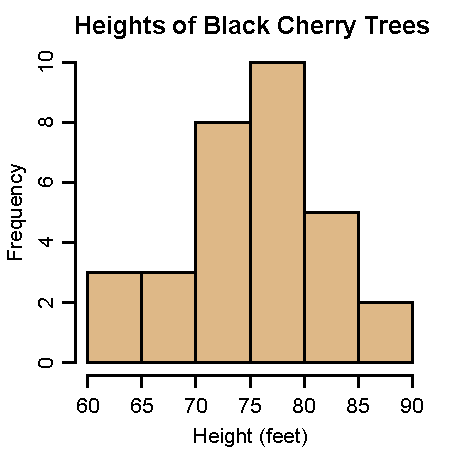
\includegraphics[width=6cm]{Black_cherry_tree_histogram.pdf}
		\caption{Black cherry tree histogram. Source: Wikimedia Commons.}
		\label{fig:histo-variabilite}
	\end{center}
\end{figure}


Puis décrivez la manipulation que vous avez effectuée pour montrer qu'une grande part de cette variabilité provient de la stochasticité de l'algorithme. 


\subsection{Influence de la charge système}
En vous appuyant sur le cours, expliquez pourquoi le temps CPU, bien que fait pour être le plus indépendant possible de la charge système, peut tout de même être influencé par la charge système en pratique. Décrivez l'expérience que vous avez effectuée pour tester cet effet et synthétisez-en les résultats, en appuyant vos affirmations sur des chiffres. 

\subsection{Influence des options de compilation}
Quantifiez le gain de performance obtenu en passant d'une compilation en mode debug à une compilation en mode release (option d'optimisation) : indiquez le pourcentage d'amélioration ainsi que la façon dont vous l'avez calculé (formule, mais aussi nombre de runs, etc).
